\documentclass[12pt,a4paper]{article}
% Set paper dimension
\usepackage[
  top=2cm,
  bottom=2cm,
  left=2cm,
  right=2cm,
  headheight=17pt, % as per the warning by fancyhdr
  includehead,includefoot,
  heightrounded, % to avoid spurious underfull messages
]{geometry}
\usepackage[english]{babel}
\usepackage[utf8]{inputenc}
\usepackage{graphicx}
\graphicspath{ {images/} }
\usepackage{amsmath}
\usepackage{mathtools}
\usepackage{amsfonts}
\usepackage{amssymb}
\usepackage{fancyhdr}
\usepackage{wrapfig}
\usepackage{lscape}
\usepackage{rotating}
\usepackage{epstopdf}
\usepackage{glossaries} 
\usepackage{float}

\usepackage{multicol}
\usepackage{paralist}
\usepackage{titlesec}
\usepackage{hyperref}

\title{Software Design Document}


% For the revision table
\usepackage[table]{xcolor}
\setlength{\arrayrulewidth}{0.5mm}
\setlength{\tabcolsep}{12pt}
\renewcommand{\arraystretch}{1.5}

\renewenvironment{enumerate}[1]{\begin{compactenum}#1}{\end{compactenum}}

\usepackage{hyperref}
 % Margins
\topmargin=-0.1in

% Headings
\pagestyle{fancy}
\fancyhf{}
\rhead{\textbf{Page} \thepage}
\lhead{Software Design Document for Lunar Rover Mapping Robot}

\pagenumbering{roman}

\begin{document}
	\begin{titlepage}
		\centerline{\rule{6.5in}{4pt}}
		\vspace*{0.5in}
		\begin{center}
			{\fontfamily{cmr}\selectfont
				{\fontsize{33}{40}\selectfont \textbf{Software Design Document}}\\
				\vspace*{0.5in}
				{\fontsize{20}{40}\selectfont for}\\
				\vspace*{0.5in}
				{\fontsize{33}{40}\selectfont \textbf{Lunar Rover Mapping Robot}}\\
				\vspace*{0.65in}
				{\fontsize{18}{40}\selectfont Version 2.0}\\
				\vspace*{2.5cm}
				{\fontsize{25}{40}\selectfont \textbf{Group: UG12}}\\
				\vspace*{2.5cm}
                \begin{figure}[H]
                \centering
                
\includegraphics[width=0.5\textwidth]{UofA.jpg}
              \end{figure}
              \vspace*{\fill}
			}
		\end{center}
		\centerline{\rule{6.5in}{4pt}}
	\end{titlepage}
	
	\newpage
	
	\tableofcontents
	
    \newpage
   	
	\noindent{\fontsize{16}{40}\textbf{Revision History}}
	\begin{center}
	\begin{tabular}{ |p{2cm}|p{3cm}|p{9cm}|  }
	\hline
	\rowcolor{lightgray}
	Version & Date &Reason for changes \\
	\hline
	1.0 & 3/10/2017 &Initial draft \\
    \hline
	2.0 & 28/10/2017 &Final version \\
	\hline
	\end{tabular}
	\end{center}
    
    \vspace{50px}
    \listoffigures

	\newpage
	
    	\pagenumbering{arabic}

\section{Introduction}

\subsection{Purpose}
This document details the software design for the Lunar Rover Mapping Robot Project. It presents the detailed description of the system and will explain system architecture and module design. This document is a guide for building the system of the project.
\subsection{Scope}
This document contains a complete description of the design of the Lunar Rover Mapping Robot Project to satisfy the requirements as specified in Software Requirement Specification. 
\subsection{References}
    \hypertarget{googlelunarxprize}{[1] Google Lunar XPRIZE. 2017. \emph{Google Lunar XPRIZE}. [ONLINE] Available at: \url{https://lunar.xprize.org}. [Accessed 4 September 2017].}\\
\subsection{Overview}
The Software Design Document is divided into 7 sections.  The sections are listed below:

\begin{enumerate}
  \item System Overview \\
  This section gives the overview of the system.
  \item System Architecture and Components Design \\
  This section describes the whole architecture and component designed of the system.
  \item Data Design \\
  This section describes how the data is stored and its representation in the system.
  \item Design Details \\
  This section gives the detail of the class design in the system.
  \item Human Interface Design \\
  This section describes the design details of the User Interface.
  \item Resource Estimates \\
  This section lists the requirements of the computer resource estimation for operating the system.
  \item Definitions, Acronyms, and Abbreviations \\
  This section lists all the definitions, acronyms and abbreviations that used in this document
  
  
\end{enumerate}

\subsection{Constraints}
The biggest constraint in the design and implementation of the system is time. The allocated time is roughly 3 months for design, development, testing and documentation of both the hardware and software components of the project. A significant portion of the allocated time would be spent on  the team becoming familiar with the development tools to aid in the development of the system. Furthermore, the team only have access to one robot unit which makes the development of the system a challenge due to the fact that each sub group in the team doing different parts of the project needs to take turns in gaining access to the robot.

\section{System Overview}
The system is comprised of three modules: the UI, Handler, and Robot. The UI provides a graphical user interface for receiving commands from users and showing information which is fetched from the Handler. The Handler handles event commands, sensor data transfers and provides path finding. The Robot manages the low-level functionality and sends sensor data to the Handler. Queues are used to communicate messages between each module.

\newpage
\section{System Architecture and Components Design}
\subsection{Architectural Description}
The software consists of three primary modules, named \textbf{UI}, \textbf{Handler}, and \textbf{Robot}, in addition to a \textbf{Map} data structure. The UI is responsible for displaying information to the user through a graphical user interface (GUI), and providing user input information to the Handler. The Handler is responsible for taking information from the UI and Robot modules, making high-level decisions, and communicating commands to the Robot. The Handler is responsible for tasks such as pathfinding and processing sensor data to be stored into the Map data structure, which holds the information about the surveyed area. The Robot component translates high-level motion commands to actuation of motors, and communicates processed sensor data back to the Handler.

\begin{figure}[H]
	\caption{An overview of the system components.}
	\centering
		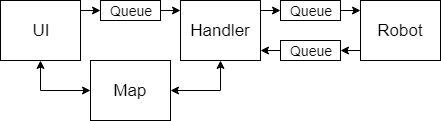
\includegraphics[width=0.6\textwidth]{SystemBlockDiagram.png}
\end{figure}

Commands and messages are communicated between modules through the use of queue objects. This is so the system can easily be modified to be multithreaded if required.

\subsection{Component Decomposition Description}
	The main components (\textbf{UI}, \textbf{Handler}, and \textbf{Robot}) have been divided up into several subcomponents, as well as several small components that exist outside of or are shared between them. The \textit{Application} component controls each of the main components, setting them up at system startup and managing their behaviour. The \textit{Map} component contains information about the surveyed location and is shared between parts of the UI and Handler. Three queues are used to communicate between high-level modules: \textit{UIEventQueue}, \textit{HandlerToRobotQueue}, and \textit{RobotToHandlerQueue}.

\subsection{Detailed Components Design Description}

\subsubsection{User Interface}
	\textbf{Purpose:} Satisfies user interface requirements (SRS Section 5.1).\\
	\textbf{Function:} This component displays the user interface for the user. It communicates UI events, such as a key or on-screen button press, to the Handler module.\\
	\textbf{Subordinates:} UIEventQueue, Map, Handler\\
	\textbf{Dependencies:} Must place UI events onto the UIEvent Queue.\\
	\textbf{Interfaces:} The component receives input from the user, and reads information from the Map and Handler. The component sends information to the Handler through the UIEventQueue.\\
    
\subsubsection{Handler}
	\textbf{Purpose:} Partly satisfies user requirements SF01 (Manual Control) and SF02 (Autonomous Control), along with the Robot.\\
	\textbf{Function:} Processes sensor data received from the Robot and UI events received from the User Interface. Updates the Map data structure and communicates commands to the Robot.\\
	\textbf{Subordinates:} Map, UIEventQueue, HandlerToRobotQueue, RobotToHandlerQueue\\
	\textbf{Dependencies:} Must send commands to the robot through the HandlerToRobotQueue.\\
	\textbf{Interfaces:} Sends and receives data to and from the Robot through \textit{HandlerToRobotQueue} and \textit{RobotToHandlerQueue} respectively. Receives data from the UI through \textit{UIEventQueue}. Processes and stores Robot sensor data in the \textit{Map}.\\
    \textbf{Data:} Stored in the \textit{Map} data structure. Also stores some robot properties, such as position and direction.\\

\subsubsection{Robot}
	\textbf{Purpose:} Partly satisfies user requirements SF01 (Manual Control) and SF02 (Autonomous Control), along with the Handler.\\
	\textbf{Function:} Received high-level commands from the Handler and translates them into motor actuation. Sends sensor data to the Handler.\\
	\textbf{Subordinates:} HandlerToRobotQueue, RobotToHandlerQueue\\
	\textbf{Dependencies:} Must send status and sensor data to the Handler through RobotToHandlerQueue.\\
	\textbf{Interfaces:} Sends data to the Handler through RobotToHandlerQueue and receives data from the Handler through HandlerToRobotQueue.\\
    \textbf{Data:} Stores handles for the component motors and various data describing the robot state, including current position and direction.\\

\subsubsection{Map}
	\textbf{Purpose:} Satisfies user requirement SF03 (Mapping), along with the ColorSensorInterpreter and DistanceSensorInterpreter components.\\
	\textbf{Function:} Stores the location of features detected by the Robot.\\
	\textbf{Subordinates:} N/A\\
	\textbf{Dependencies:} N/A\\
	\textbf{Interfaces:} Allows methods to retrieve feature likelihoods (how probable there is a feature at a location) at a given position and set feature likelihoods at any position. Also provides some utilities to get colours at a position (using an assigned colour table for features) and get the most likely feature at a position.\\
    \textbf{Data:} Stores a matrix of likelihoods for each possible feature in the map. The grid size of each element in the matrix (in metres) is specified when the Map is created.\\

\subsubsection{UIEventQueue}
	\textbf{Purpose:} Aids in satisfying requirements through the UserInterface and Handler components, and the performance requirement NF-R02 (Real-Time Communication).\\
	\textbf{Function:} Communicates UI input events to the Handler module.\\
	\textbf{Subordinates:} UserInterface, Handler\\
	\textbf{Dependencies:} N/A\\
	\textbf{Interfaces:} Allows messages to be added and removed\\
    \textbf{Data:} Stores the messages as a FIFO queue.\\
    
\subsubsection{HandlerToRobotQueue}
	\textbf{Purpose:} Aids in satisfying requirements through the Handler and Robot components, and the performance requirement NF-R02 (Real-Time Communication).\\
	\textbf{Function:} Communicates high-level commands from the Handler to the Robot.\\
	\textbf{Subordinates:} Handler, Robot\\
	\textbf{Dependencies:} N/A\\
	\textbf{Interfaces:} Allows commands to be added and removed.\\
    \textbf{Data:} Stores the commands as a FIFO queue.\\
    
\subsubsection{RobotToHandlerQueue}
	\textbf{Purpose:} Aids in satisfying requirements through the Handler and Robot components, and the performance requirement NF-R02 (Real-Time Communication).\\
	\textbf{Function:} Communicates robot state and sensor data from the Robot to the Handler.\\
	\textbf{Subordinates:} Handler, Robot\\
	\textbf{Dependencies:} N/A\\
	\textbf{Interfaces:} Allows messages to be added and removed.\\
    \textbf{Data:} Stores the messages as a FIFO queue.\\
    
\subsubsection{ColorSensorInterpreter}
	\textbf{Purpose:} When used with the map, satisfies user requirement SF03 (Mapping).\\
	\textbf{Function:} Translates sensed colours from the Robot's colour sensor into detected features.\\
	\textbf{Subordinates:} Map\\
	\textbf{Dependencies:} Must store interpreted data into the Map.\\
	\textbf{Interfaces:} Provides methods to assign colors to features and translate a sensed color into a feature, and store that feature into a Map.\\

\subsubsection{DistanceSensorInterpreter}
	\textbf{Purpose:} When used with the map, satisfies user requirement SF03 (Mapping).\\
	\textbf{Function:} Translates sensed distances from the Robot's ultrasonic sensor into an obstacle at a certain position.\\
	\textbf{Subordinates:} Map\\
	\textbf{Dependencies:} Must store interpreted data into the Map.\\
	\textbf{Interfaces:} Provides a method to translate a sensed distance into a position in the Map, and store an obstacle feature at that position.\\

\subsubsection{PathFinding}
	\textbf{Purpose:} This component when used with the Map component satisfies the user requirement SF02 (Autonomous Control).\\
	\textbf{Function:} Finds the shortest path from the Robot's position to a destination point on the map while avoiding any impassable areas.\\
	\textbf{Subordinates:} Map, Node\\
	\textbf{Dependencies:} The found path must be within the map.\\
	\textbf{Interfaces:} Receives a Cartesian coordinates of the current position of the Robot and the destination point from the Handler and returns the shortest path, which is a collection of Cartesian coordinates, between the two points.\\
    \textbf{Data:} The estimated travel cost from the Robot's position to each inspected grid then to the destination point.\\
    
\subsubsection{Node}
	\textbf{Purpose:} This component when used with the PathFinding component assists in satisfying the user requirement SF02 (Autonomous Control).\\
	\textbf{Function:} Stores the estimated costs \textit{g} (the cost to travel from the Robot's position to this node/point), \textit{h} (the displacement cost between this point and the destination point) and \textit{f} (the total cost, i.e. \textit{h} + \textit{g}) and its adjacent nodes which are used by the PathFinding component to find the shortest path.\\
	\textbf{Subordinates:} Point\\
	\textbf{Dependencies:} N/A\\
	\textbf{Interfaces:} Calculates and stores the estimated costs and sends it to the PathFinding component when it is needed.\\
    \textbf{Data:} The estimated costs and this node's adjacent nodes.\\

\subsection{Architectural Alternatives}
Aside from our modular, communication queue-based approach, we also considered a layered architecture. With this architecture, our independent modules (UI, Handler, and Robot) would be replaced with a stack of software layers from high-level (the user interface), through intermediate layers (the equivalent of the Handler module), with the lowest level being direct control of the actuation of the robot motors.

\subsection{Design Rationale}
We decided on using the communication queue-based architecture over the layered architecture due to the difference in the ease of switching each architecture to a multithreaded variant. When analysing the software requirements, we found that a multithreaded system may be required to stop high-level logic from blocking low-level controls and preventing quick responses to environmental changes at a low level, e.g. stopping the robot before it collided with an obstacle. A layered approach would be difficult to arrange in such a way that it could be easily split into several independent threads of execution. However, the approach of using communication queues means that our design can be modified to have any of the three main components (UI, Handler, and Robot) moved into a separate thread of execution using a thread-safe queue object. This means that our communication queue method is more robust to this architectural change if it was required.

\newpage
\section{Data Design}
\subsection{Database Description}
The system must store the data that the robot has sensed into some representation of the surveyed location. To do this, we have designed a \textit{Map} data structure which stores a grid of likelihoods for each feature that is required to be detected by the robot.

\subsection{Data Structures}
The \textit{Map} consists of a number of stacked matrices, one for each feature (or \textit{property} in the codebase) that the robot can detect. Each matrix has the same dimensions. The surveyed location is divided up into a grid,  and the elements in each matrix correspond with a square in the grid. When the Map is initialized, the grid dimensions (in \textit{rows} and \textit{columns}) and grid element size (in \textit{metres}) are specified.
Each element in each matrix contains a value varying between 0.0 and 1.0. This value represents a likelihood that a feature is present in this grid element. This allows the Handler logic to account for sensor error when utilizing the Map data.

The Map provides utilities to convert from points in metre coordinates to locations in the Map grid, and to retrieve and set values in the Map. It can also determine the most likely feature at a position.

\begin{figure}
	\caption{The Map data structure represented as a UML class diagram. \textit{n} is the number of features (or properties) the Map can store.}
	\centering
		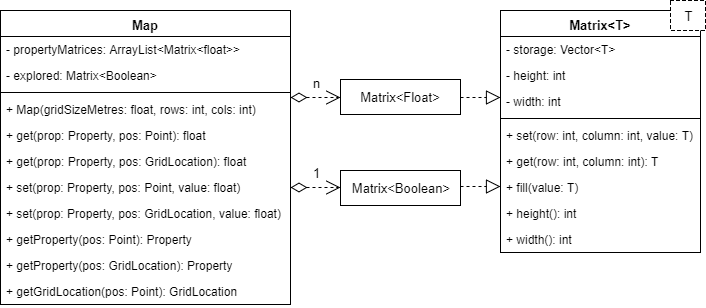
\includegraphics[width=1.0\textwidth]{MapDataStructure}
\end{figure}

\section{Design Details}
\subsection{Class Diagrams}
See figure \ref{fig:class_diagram} at the end of the document.

\subsection{State diagrams}
As the Handler and Robot are separate modules, they are presented as two different state machines. The UI does not have any state, as it is implemented through the Java event system.
\begin{figure}[H]
	\caption{The state diagram for the Handler component}
	\centering
		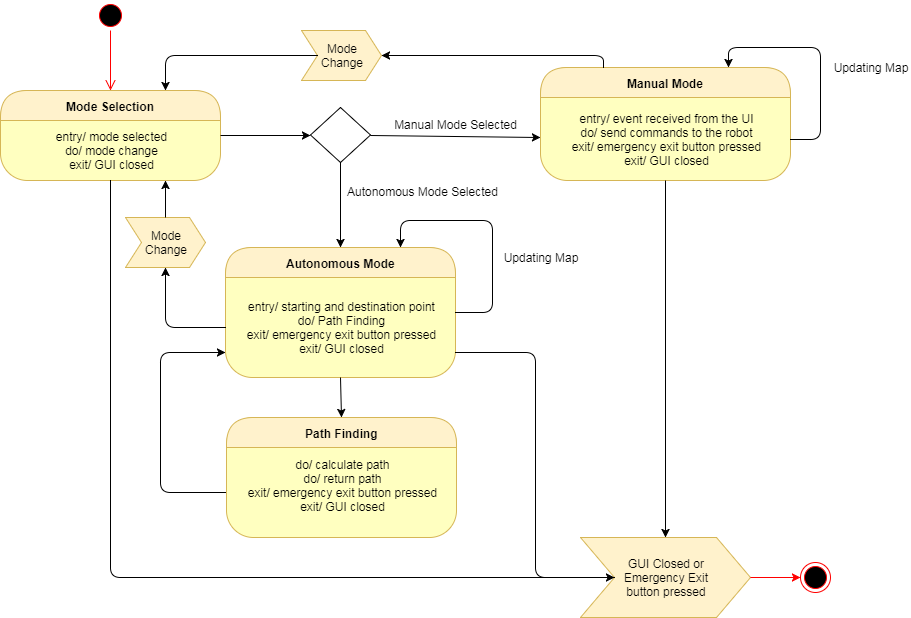
\includegraphics[width=1.0\textwidth]{HandlerState.png}
\end{figure}
\begin{figure}[H]
	\caption{The state diagram for the Robot component}
	\centering
		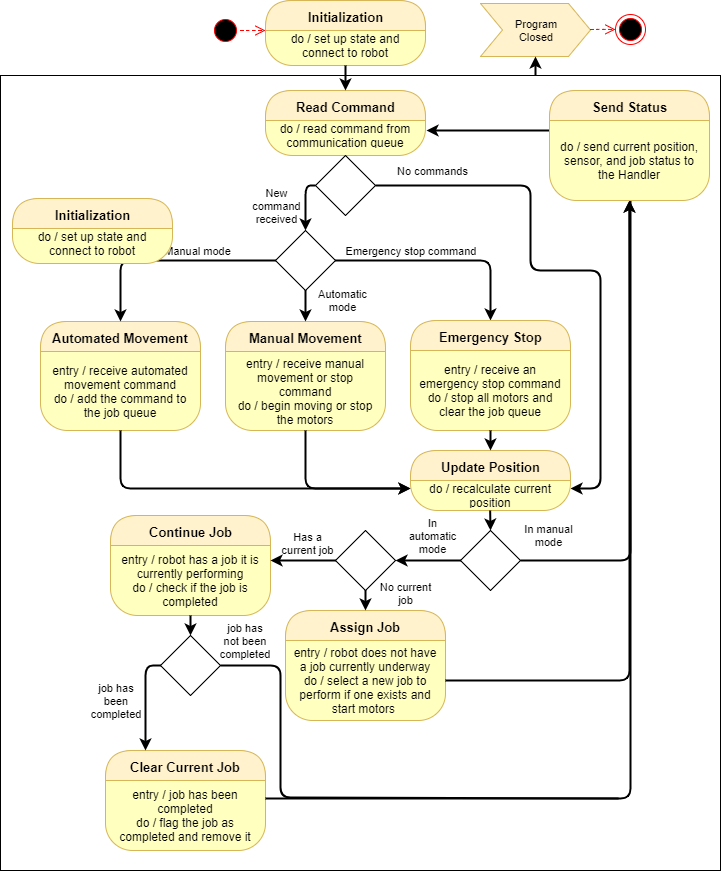
\includegraphics[width=0.9\textwidth]{RobotState.png}
\end{figure}

\subsection{Interaction Diagrams}
\begin{figure}[H]
	\caption{The interaction diagrams for user requirements SF01 and SF02.}
	\centering
		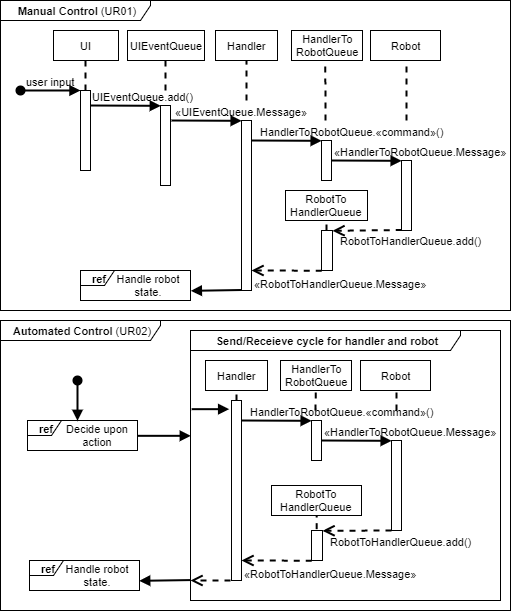
\includegraphics[width=0.8\textwidth]{Interactions.png}
\end{figure}
\newpage
\section{Human Interface Design}
\subsection{Overview of the User Interface}
The User Interface is implemented based on MVC (Model View Controller) software architecture pattern.  User can interact with the software through the GUI, which facilitates user’s utilization of program. The GUI provides buttons to allow user operating the software by clicking on it or press the key. And the data of map structure will be rendered to a region of GUI which will display the visualization of map data.\\
\subsection{Detailed Design of the User Interface}
There are two screens of GUI. One is connection screen and another one is the general screen. The connection screen is displayed at the launch of the program. It asks user to enter the IP address to connect robot. General screen will show up to the user once the connection is built. \\
\begin{itemize}
\item 
The Connection Screen of GUI has mainly two parts. The message panel will display the current status of the connection and the selection panel allows user to select the connection mode\\
\begin{figure}[!htb]
\centering
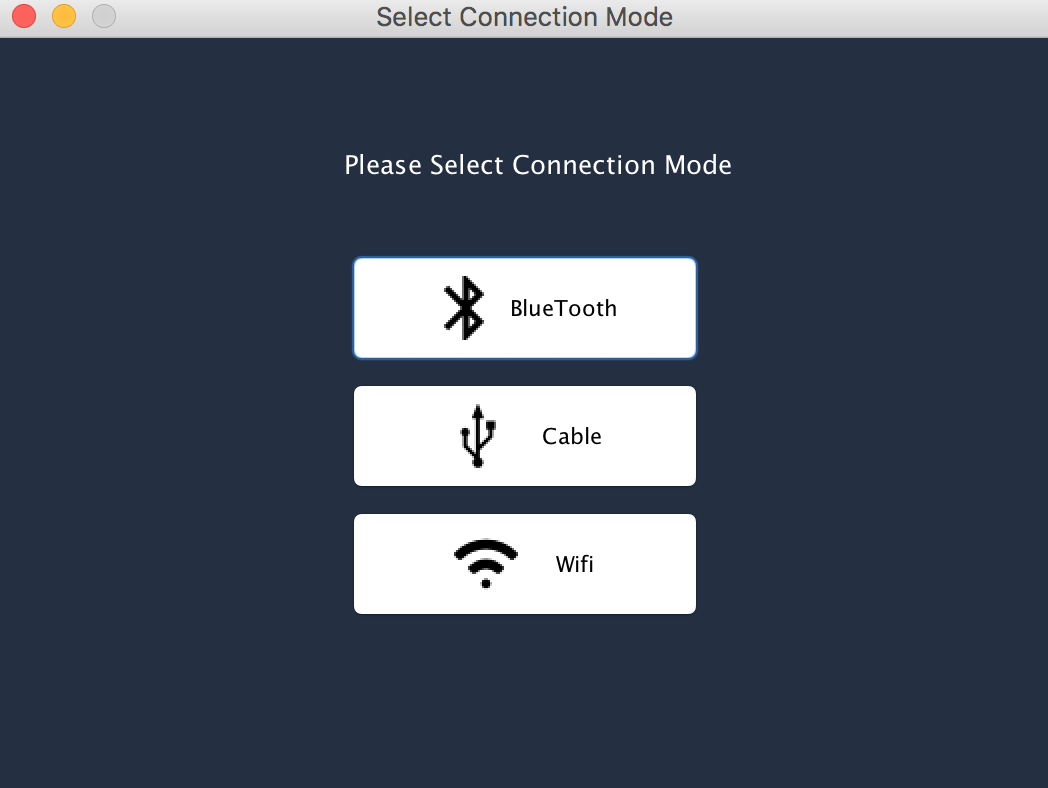
\includegraphics[width=0.4\textwidth]{ConnectionPage}
\caption{Connection Screen} 
\end{figure}

\begin{itemize}
\item "Bluetooth" button should be selected by click when the connection is via Bluetooth. Robot will have the IP address 10.0.1.1.
\item "Cable" button should be selected by click when the connection is via cable. Robot will have the IP address 10.0.1.1.
\item "WiFi" button should be selected by click when the connection is via WiFi. The robot will be assigned an IP address and it is displayed on the brick screen. It will pop up a prompt to ask User enter the IP address.

\end{itemize}

\newpage

\item
The are mainly three sections on the general screen which are map panel, control panel and switch panel. \\
\begin{figure}[!htb]
\centering
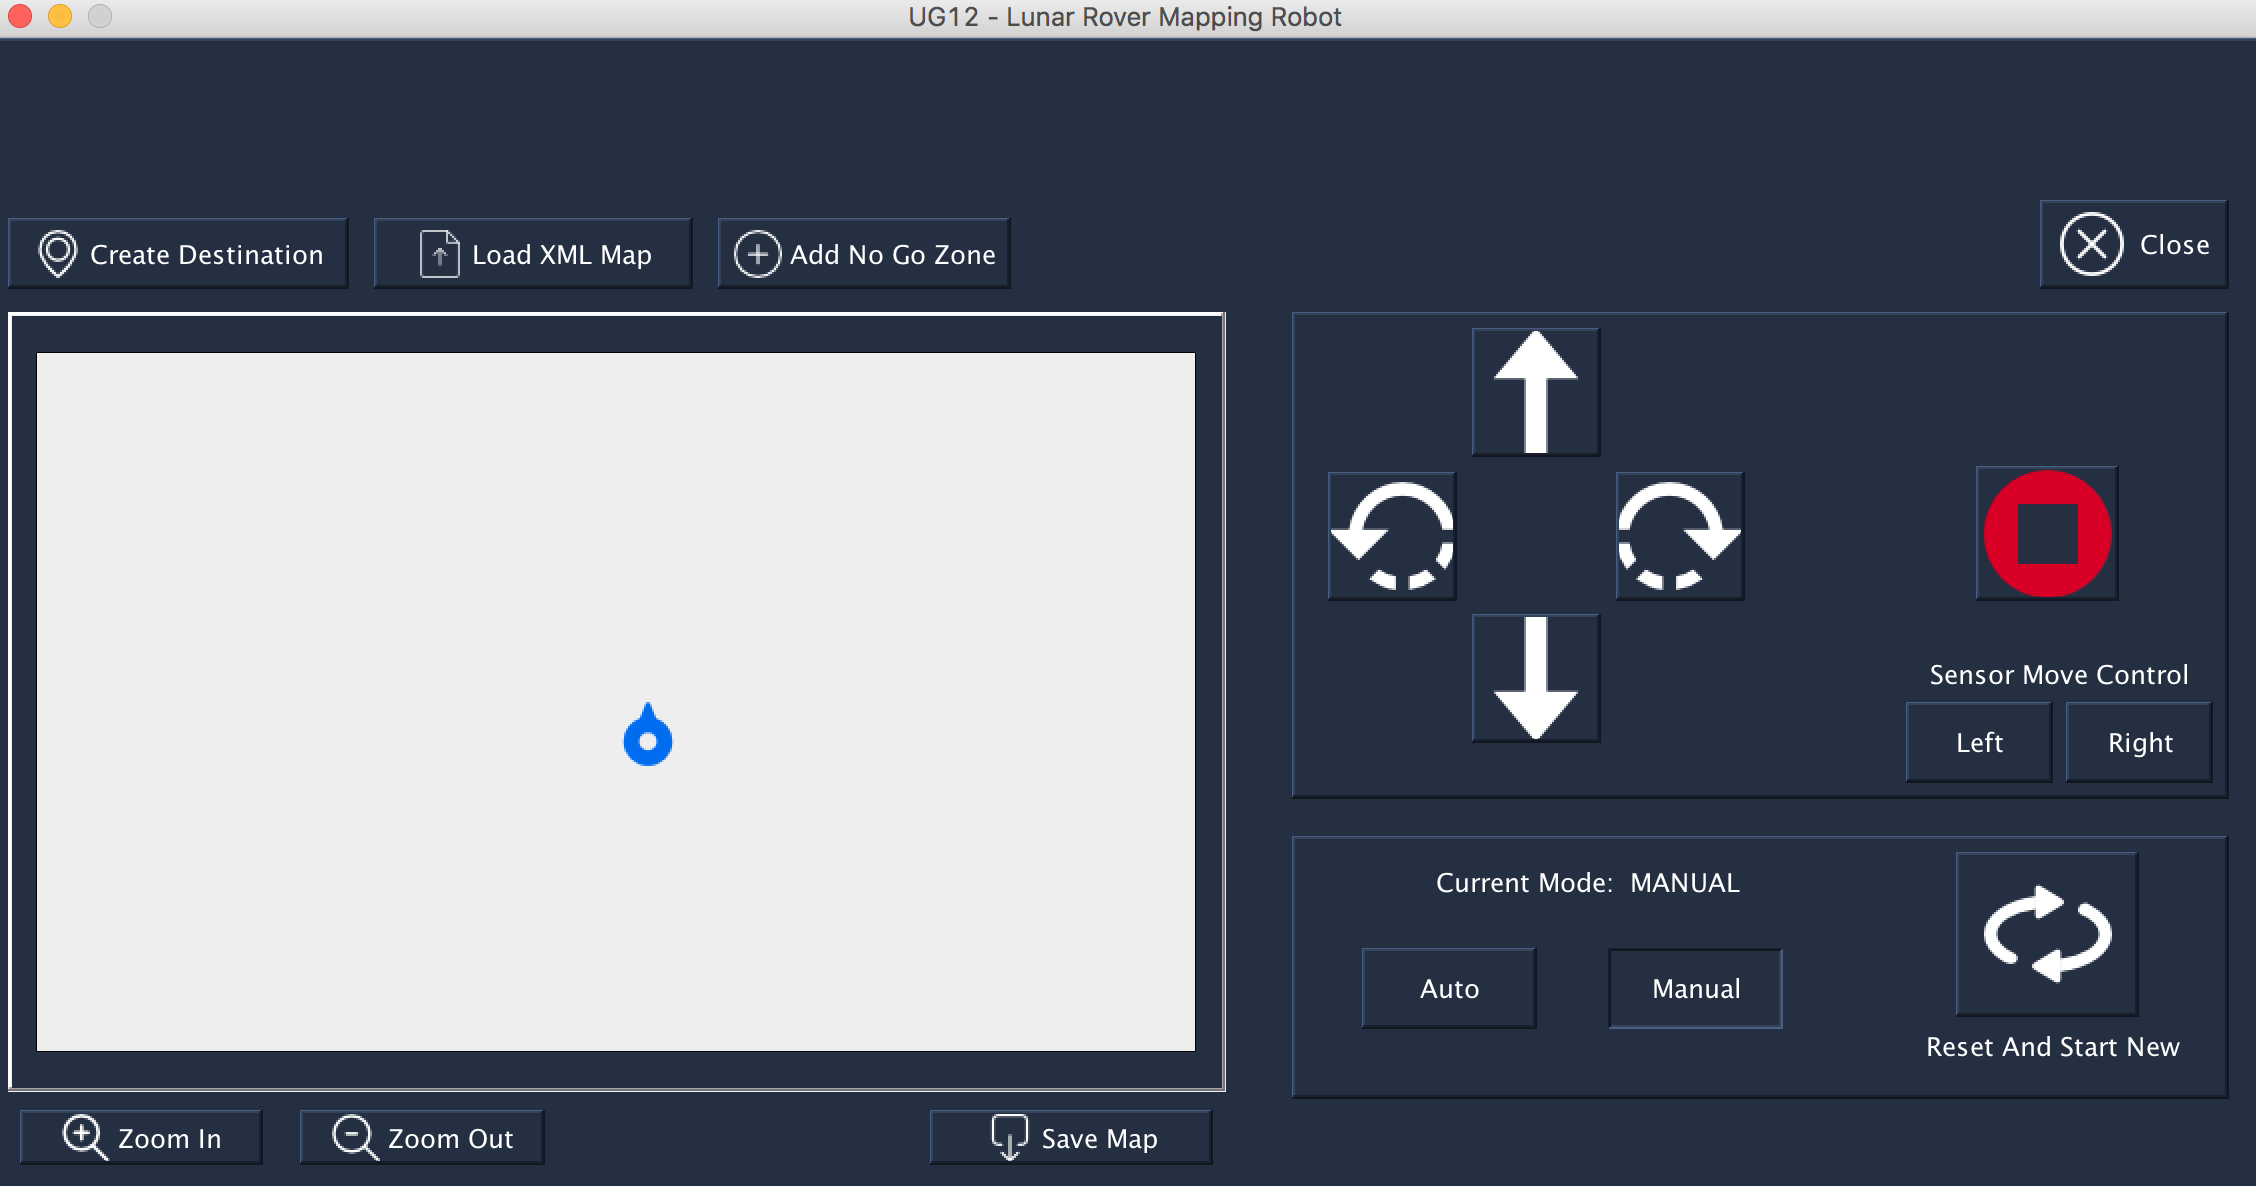
\includegraphics[width=0.4\textwidth]{GeneralPage}
\caption{General Screen} 
\end{figure}

\titleformat{\paragraph}
{\normalfont\normalsize\bfseries}{\theparagraph}{1em}{}
\titlespacing*{\paragraph}
{0pt}{3.25ex plus 1ex minus .2ex}{1.5ex plus .2ex}

\item Control Panel - Robot movement control (SF01 Manual Control)
\begin{figure}[!htb]
\centering
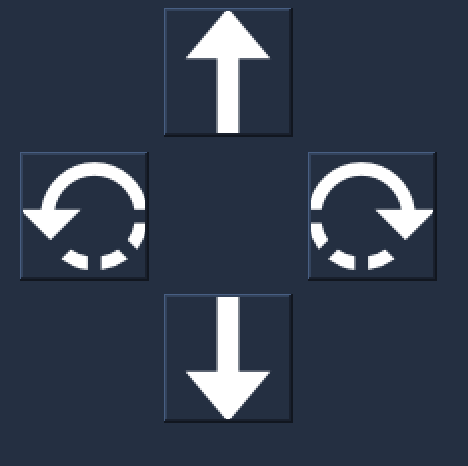
\includegraphics[width=0.2\textwidth]{ControlPanel}
\caption{Moving Control} 
\end{figure}
\begin{itemize}
\item The button with up arrow will send forward command when user click on it or press up arrow key on the keyboard. 
\item The button with down arrow will send backward command when user click on it or press down arrow key on the keyboard. 
\item The button with left rotate arrow will send left rotate command when user click on it or press left arrow key on the keyboard. 
\item The button with right rotate arrow will send right rotate command when user click on it or press right arrow key on the keyboard. 
\end{itemize}

\item Control Panel - Colour Sensor movement
\begin{figure}[!htb]
\centering
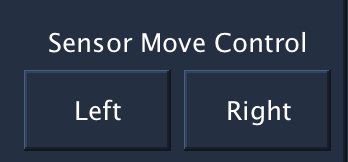
\includegraphics[width=0.2\textwidth]{SensorMove}
\caption{Colour Sensor Move Control} 
\end{figure}

\begin{itemize}
\item The left button will send left moving command to move left the colour sensor when user click on it or press "A".
\item The right button will send right moving command to move right the colour sensor when user click on it or press "D".
\end{itemize}

\item Control Panel - Emergency Stop (SF01 Manual Control)
\begin{figure}[!htb]
\centering

\includegraphics[width=0.1\textwidth]{EmergencyStop}
\caption{Emergency Stop} 
\end{figure}
\begin{itemize}
\item The button will send emergency stop command to the robot to stop the robot from movement immediately.
\end{itemize}

\item Switch Panel - Automatic and Manual Switch (R01 Manual Control and R02 Autonomous Control)\\
\begin{figure}[!htb]
\centering
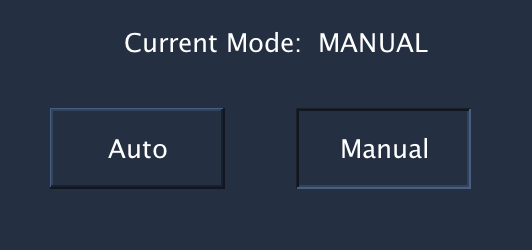
\includegraphics[width=0.3\textwidth]{AutoManualSwitcher}
\caption{ Automatic and Manual Switch} 
\end{figure}
\begin{itemize}
\item When manual button is on click, it will switch the robot to the manual mode which allows user to manually control the robot and enable sending robot movement commands.
\item When Automatic button is on click, it will switch the robot to the automatic mode which enable self path finding of the robot and disable sending robot movement commands.
\item The current mode can be viewed on the status window.
\end{itemize}

\item Switch Panel - Reset and Restart\\
\begin{figure}[!htb]
\centering
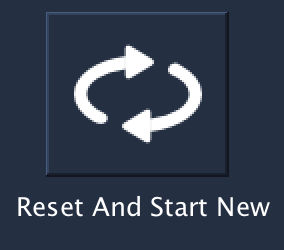
\includegraphics[width=0.2\textwidth]{Reset}
\caption{Reset and Restart} 
\end{figure}
\begin{itemize}
\item When the robot has reached the destination, The reset button allows User has the option to reset the figures of map.
\end{itemize}

\item Map Panel - Map display region (SF03 Mapping)\\
\begin{figure}[!htb]
\centering
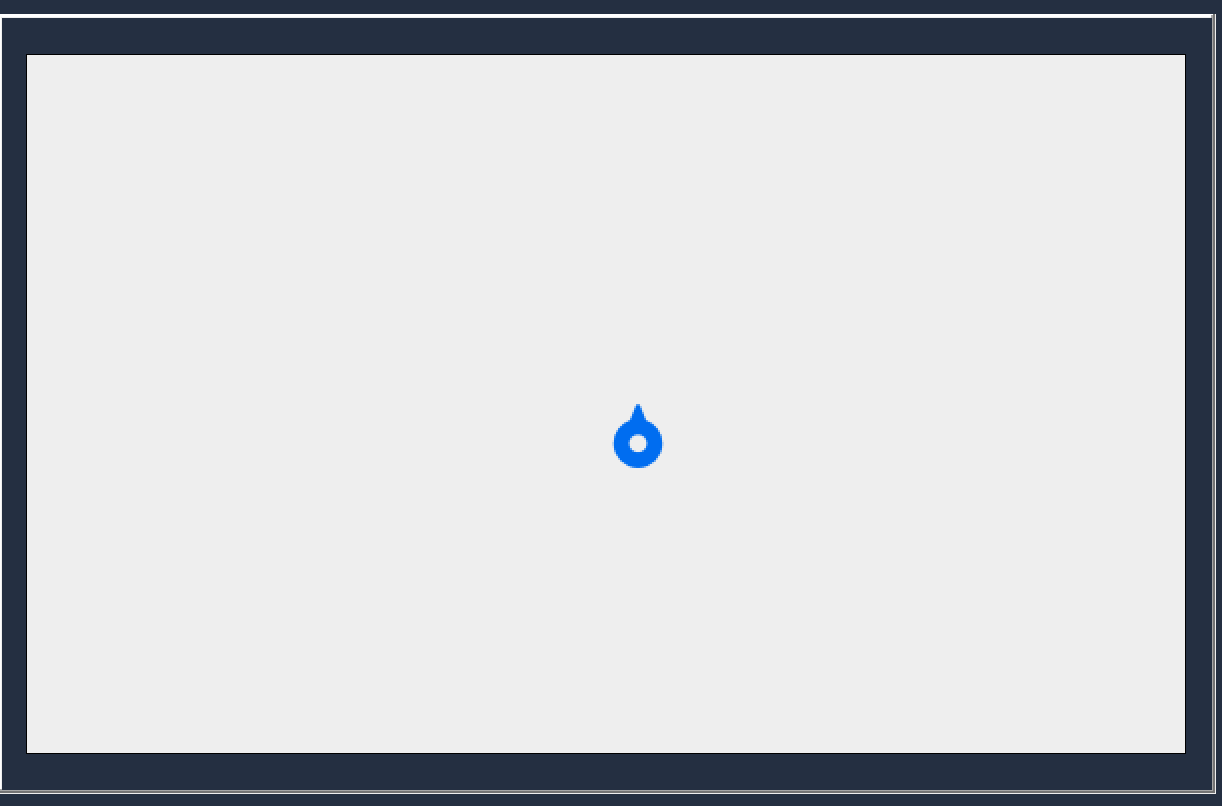
\includegraphics[width=0.4\textwidth]{MapDisplay}
\caption{Map Display} 
\end{figure}
\begin{itemize}
\item This region will display the map visualization by rendering the map data. It displays the robot position and map features. It also allow user to modify the map by marking no go zones or creating destination. 
\end{itemize}

\item Map Panel - Map Editing Buttons (SF03 Mapping)\\
\begin{figure}[!htb]
\centering

\includegraphics[width=0.5\textwidth]{MapEditing}
\caption{Map Editing buttons} 
\end{figure}
\begin{itemize}
\item The map editing buttons are placed on the top of the map display region. They have the functionalities to allow user modify the map.
\item When user click on "Create Destination" button, it allows user to create a destination by clicking the specific point on map. Then the text on this button will become "confirm", user needs to click on it to confirm the destination.
\item When user click on "Load XML map" button, it allows user to load the data of DTD.xml into the map structure. The DTD.xml will also be rendered and displayed to user at the same time.
\item When user click on "Add No Go Zone", It allows user to mark the NGZs on the map. User can use the mouse to drag a shape on the map display region. Then the text on this button will become "confirm", user needs to click on it to confirm the NGZs.
\end{itemize}

\item Map Panel - Zoom In/Out\\
\begin{figure}[!htb]
\centering

\includegraphics[width=0.5\textwidth]{Zoom}
\caption{Zoom In/Zoom Out} 
\end{figure}
\begin{itemize}
\item One click on "Zoom in" button will enlarge the components displayed in the map 1.1 times bigger.  
\item One click on "Zoom out" button will narrow the components displayed in the map 1.1 times smaller.
\item When the map is zoomed in, user can click on the map to move the camera. 
\end{itemize}

\item Map Panel - Save Map (SF03 Mapping) \\
\begin{figure}[!htb]
\centering

\includegraphics[width=0.3\textwidth]{Save}
\caption{Save Map} 
\end{figure}
\begin{itemize}
\item "Save Map" Button allows user to save the data of current map. All features of the map will be rendered into format. 
\end{itemize}

\item Close\\
\begin{itemize}
\begin{figure}[!htb]
\centering

\includegraphics[width=0.2\textwidth]{Close}
\caption{Close Button} 
\end{figure}
\item When use click on close button, it will send command to close all the motor and sensor ports and then exit the program.
\end{itemize}
\end{itemize}



\newpage
\section{Resource Estimates}
The program is not computationally intensive, and does not require a large amount of space. Any modern computer system should have sufficient CPU, GPU, RAM, and HDD space to run this program. 500MB of RAM, and 200MB of HDD space should be sufficient.\\
The program requires Java 7 to run, and a WiFi adapter to remotely connect to the EV3 brick used in the Lunar Rover.    

\section{Definitions, Acronyms, and Abbreviations}
\textbf{CPU}: Central Processing Unit\\
\textbf{GPU}: Graphics Processing Unit\\
\textbf{GUI}: Graphical User Interface\\
\textbf{HDD}: Hard Disk Drive\\
\textbf{RAM}: Random Access Memory\\
\textbf{SDD}: Software Design Document\\
\textbf{SPMP}: Software Project Management Plan\\
\textbf{SRS}: Software Requirements Specification\\
\textbf{UI}: User Interface\\

  
\begin{sidewaysfigure}[!htb]
    	\centering
        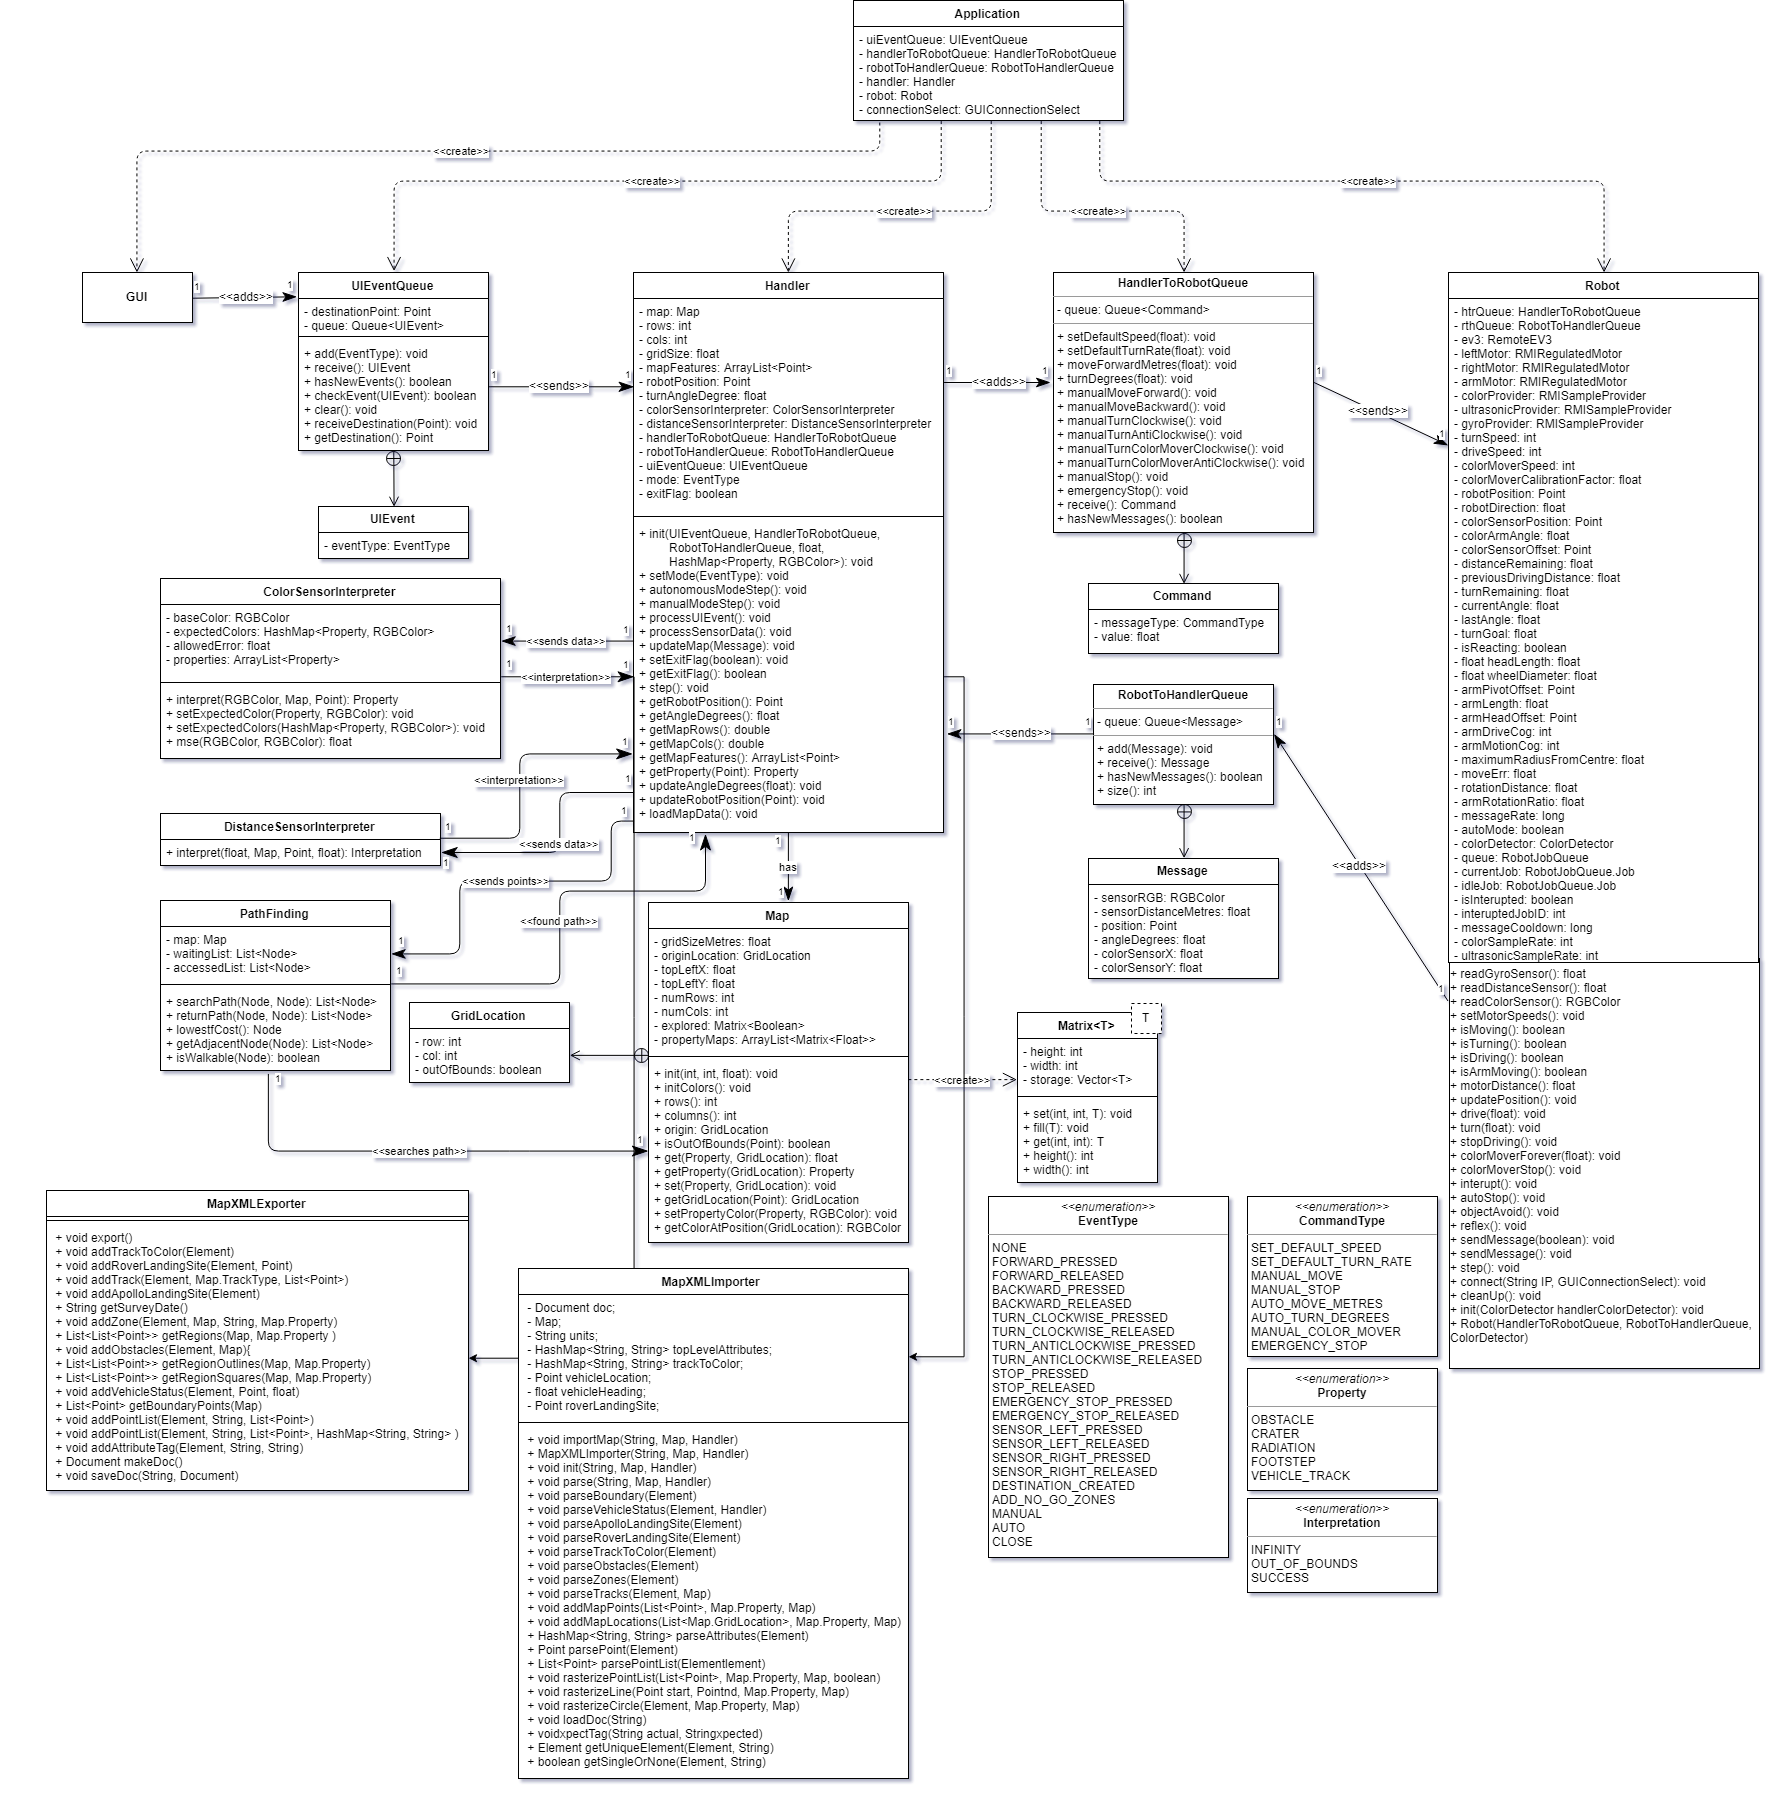
\includegraphics[width = 24cm, height = 16cm]{Class_Diagram_2.png}
    	\caption{Class Diagram}
        \label{fig:class_diagram}
\end{sidewaysfigure}


\end{document}
 